\chapter{Experiment}

This chapter presents the experimental environment used in order to test our hypothesis. The first two sections will focus on discussions around the choices of data domain and the CNN architecture. The next section explains all the networks variants, techniques and parameters used during the training process. The two subsequent sections are dedicated into explaining the reasons behind the chosen perturbation method and the synthetic generation of the imbalanced dataset, which are the core ideas behind this work. Finally, we link each experiment(s) with the hypothesis it tries to answer. 
\section{Data domain}

Improvements on Computer Vision were possible due to two main reasons: increased computational power and standardized datasets for benchmarking. The ever increasing amount of image data on the Internet fostered more sophisticated and robust algorithms to work on images and multimedia data. ImageNet is a large-scale ontology of images with 1.000 different classes and with 3.2 million 224x224 high resolution images in total \cite{deng2009imagenet}. CIFAR, on the other hand, is a more compact dataset with 32x32 colour images in 10 or 100 classes. The dataset consists of 60.000 images with equal amount of samples per class \cite{krizhevsky_2009}.

Even though both datasets differ on image sizes and number of class labels, they share similar data domain. CIFAR can be seen as a subset of ImageNet dataset, therefore, convolutional filters from the latter could be used to improve performance of the former as shown by Yosinski et al.(2014). Our experiment uses a CIFAR10 full dataset on a adapted VGG16 architecture. Even that both datasets differ considerably in size, the results achieved in one should be interchangeable as the CNN architecture was adapted to accomodate the difference on the dataset size.

\section{The VGG Architecture}

As described on Chapter 2, a ConvNet is a sequence of layers where every layer transforms one volume of activations to another through a differentiable function. Three main types of layers are used to build these networks: Convolutional Layer, Pooling Layer and Fully-Connected Layer.A Convolutional Layer would compute the output of neurons that are connected to local regions in the input, an Activation layer (RELU, Sigmoid etc) applies element wise functions, the Pooling layer performs downsampling operations along the spatial dimensions of the input and, finally, the Fully-connected layer computes the class scores of the classifier. The chosen architecture should have enough layers for learning good features from the training set domain. For instance, a ConvNet Architecutre for CIFAR-10 could have the following configuration: [INPUT - CONV - RELU - POOL - FC].

Network architectures with higher accuracies have better generalization over the overall data input domain, however, adversaries are efficient into extrapolating the given domain by going to previously unseen regions of space (known as domain shift \cite{papernot2016}). For this work we had to make a choice of which network architecture would not only provide reasonable accuracy for our selected data domain (CIFAR-10) but would also be reasonable on the resource consumption. This way we can reproduce the requirements of a real world system where not only accuracy is taken into account when selecting a deep learning model.

From all networks tested on Canziani et al (2016), the VGG16-19 from Simonyan et al. (2014)  seemed to have the best trade off between accuracy and performance (inference time). The VGG architecture won the first and second places on the ILSVRC-2014 submission on the localisation and classification task.The main contribution of the VGG network was showing that the depth of the network is a critical component for good classification performance. The model can be assembled with 16 or 19 Conv/FC layers and it features an extremely homogenous architecture that only performs 3x3 convolutions and 2x2 pooling from beginning to end.

\begin{figure}[!h]
	\centering
	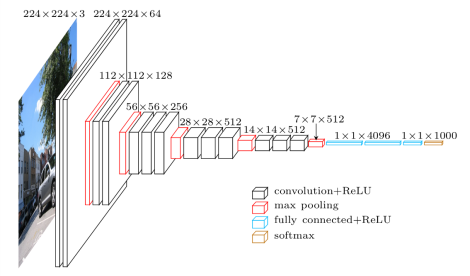
\includegraphics[scale=0.6]{imagenet_vgg16.png}
	\caption{VGG16 on ImageNet}
	\cite{simonyan2014very}
	\label{fig:vgg16}
\end{figure}

The design of the VGG16 has been proven to work even on heterogeneous datasets with several classes . The two last fully connected layers of the state of the art model are comprised of 4096 neurons each, leading to much higher parameters complexity. As the dataset used in this work has only 10 classes, the two FC-4096 layers were replaced by one single layer with 512 neurons and RELU activations. This change helped to reduce overfitting when training the network. In addition, the total number of convolutions blocks and pooling were reduced to 3, with the first layer having 2 stacked convolution layers followed by a max pooling of stride 2x2 and the last two layers with 3 stacked convolutions also followed by a max pooling of stride 2x2. The max pooling layers are responsible for reducing the image size by 50\% every time an image passes through it. Since CIFAR-10 images are only 32x32, the original VGG16 architecture would end up having an output of shape of only 1x1 pixel at the last layer. In order to avoid this problem, the number of layers were reduced so to fit our dataset domain. The resulting shape fed into the fully connected layers is 4x4x128 (Width x Height x Channels) as it can be seen on table ~\ref{tbl:vgg10}. 

\begin{table}[!h]
	\centering
	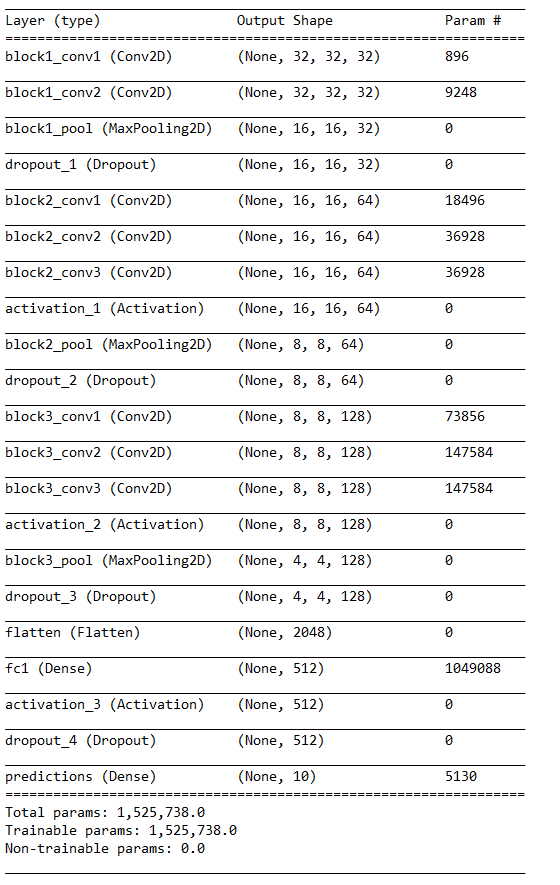
\includegraphics[scale=0.9]{vgg_arch.png}
	\caption{Full Model Description}
	\label{tbl:vgg10}
\end{table}
 
\section{Overall Training Process}

Neural Networks require good optimisation methods in order to achieve good performance. As networks get deeper, the number of resources required to train increases considerably. Convolutional Neural networks  can share parameters within its convolution layers, thus, reduce the amount of computation needed during training. All the models comprised in this work were implemented using Python programming language along with Tensorflow and Keras frameworks. The first is a high performance calculation engine that uses GPUs to accelerate its matrix/vector calculations. The latter is a Neural Network library that helps on the implementation of any deep learning model. Keras is mainly a wrapper on top of tensorflow that hides some abstraction from the developer, making it one of the best frameworks for DNNs currently.

As discussed on Chapter 2, the full gradient update would not be the best choice for optimizing deep networks. Stochastic Gradient methods were one of the first methods developed to overcome this problem and are still being further developed nowadays. The SGD based optimisation technique used in this work was developed by Bengio (2015) \cite{bengiormsprop}, namely RMSProp. This method is an adaptive learning rate scheme that can take the absolute values of the Hessian's eigenvalues and, therefore, approximate the equilibration preconditioner. As shown on Bengio's work \cite{bengiormsprop}, the method outperforms current SGD methods by achieving convergence faster.The learning rate for the method was set at $10^{-4}$ and the decay $10^{-5}$.

In order to achieve stability, every algorithm should be trained until convergence, in other words, it does no underfit or overfit the given dataset. Avoiding overfitting and underfitting is highly important when training DNNs. Our architecture was trained until no more reasonable changes were detected in the validation loss so we could dismiss unnecessary training steps and consequently any kind of overfitting. This was achieved by using the Early Stopping technique as described on \cite{stanford2016}. Fundamentally, this consists of a functional callback that runs at the end of every epoch and compares the previous loss with the current one and interrupts training if the difference was below an user provided $\delta$ for a specific number of steps in a row. The value of our $\delta$ was set at $10^{-4}$ and the number of steps to 10. For instance, training would be stopped if no improvement over the specified $\delta$ was seen for 10 steps in a row. Also, we did put a hard limit of 200 on the total number of epochs.

\begin{figure}[!h]
	\centering
	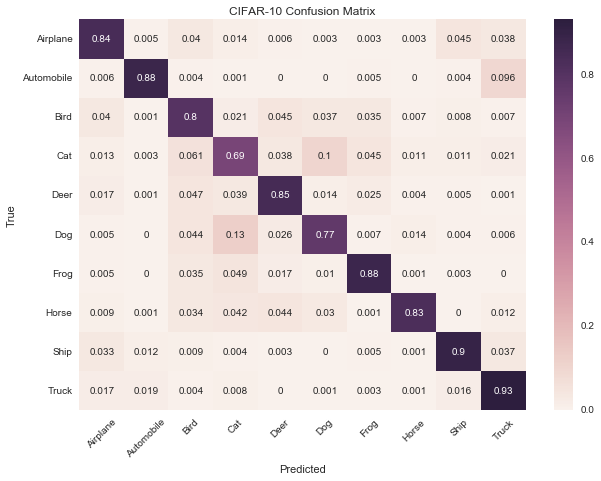
\includegraphics[scale=0.6]{conf_matrix.png}
	\caption{Results on the full dataset}
	\label{fig:conf_matrix_full}
\end{figure}

The confusion matrix helps understanding the individual score for each class and also which targets class were being misclassified into. Figure ~\ref{fig:conf_matrix} shows that the Cat and Dog classes are often interchangeably misclassified as they have a set of similar features. The network have reached an overall accuracy of 83.45\% and a total validation loss of 0.5033.

\section{Perturbation method}
Section ~\ref{sec:gsm} has shown two different types of perturbations that could be applied to images in order to generate adversaries. For instance, one could select a specific class as the target of a perturbation but this would ultimately introduce undesirable variance when crafting adversaries, as each class could have different effects within our target and, thus, the perturbation could be different on each case. In order to address this problem, we have chosen the class itself as the backpropagated gradient coupled with the ascent method. The intuition behind this choice is that we look to increase the cost function of the target class by moving away from the current label. As the class itself is chosen to cause the perturbation, our method moves to the closest data domain to our class, in other words, it follows the class own gradient uphill. For instance, cats and dogs are classes with similar feature spaces and are often misclassified among each other. A small ascent perturbation on any of these classes would most likely lead to an increase on this prior effect as both classes are occupying similar positions of the space. 

For all classes, the amount of change on each pixel needed to be carefully chosen as we did not want to change an image too much to a point where it would be unrecognizable to human perception. Moreover, in order to test our hypothesis, we needed a value that would sit on the threshold of all classes, in other words, it would be just enough to push most of the samples to the closest vicinity leading to a successful misclassification. From all the trials, the value of $\epsilon$ that seemed to fulfill our needs was 0.01. Another important choice was regarding which trained network would serve as the baseline for our gradient calculation. The balanced network was the model of choice to create all the 10 different perturbed test datasets. This is justified by the fact that the sign of the gradient is another source of variation on the Gradient Sign equation. We wanted to have similar gradient magnitudes for all classes, and that could be approximately achieved by using a network that is roughly balanced throughout all classes. All in all, the level of perturbation should not be biased towards any class and should add similar noise levels to all images.

\section{Synthetic data level imbalance}

Classification models are usually required to have similar number of samples for each class in order to equally learn proper feature representations for each label. As shown on Murphey and Guo (2004) \cite{murphey2004}, Neural Networks have lower generalization capabilities and are biased towards specific classes when trained on datasets with unequal number of samples between classes. 

As the CIFAR10 dataset is not naturally imbalanced, we have artificially created two variations on which we trained our networks.  While one dataset consisted on a direct undersample of the target class to 1.000 samples, the other was crafted using  an undersampling (or an oversampling of the target class) of all the other classes to a 1.000 samples while keeping the target class with the original number of samples (5.000). For each class of the 2 different dataset configurations, a network was then trained until convergence using the same parameters as the balanced case. Each model was evaluated against a test set of 1000 equally distributed samples perturbed by the fast gradient sign method described on the previous section. 

\begin{figure}[!h]
	\centering
	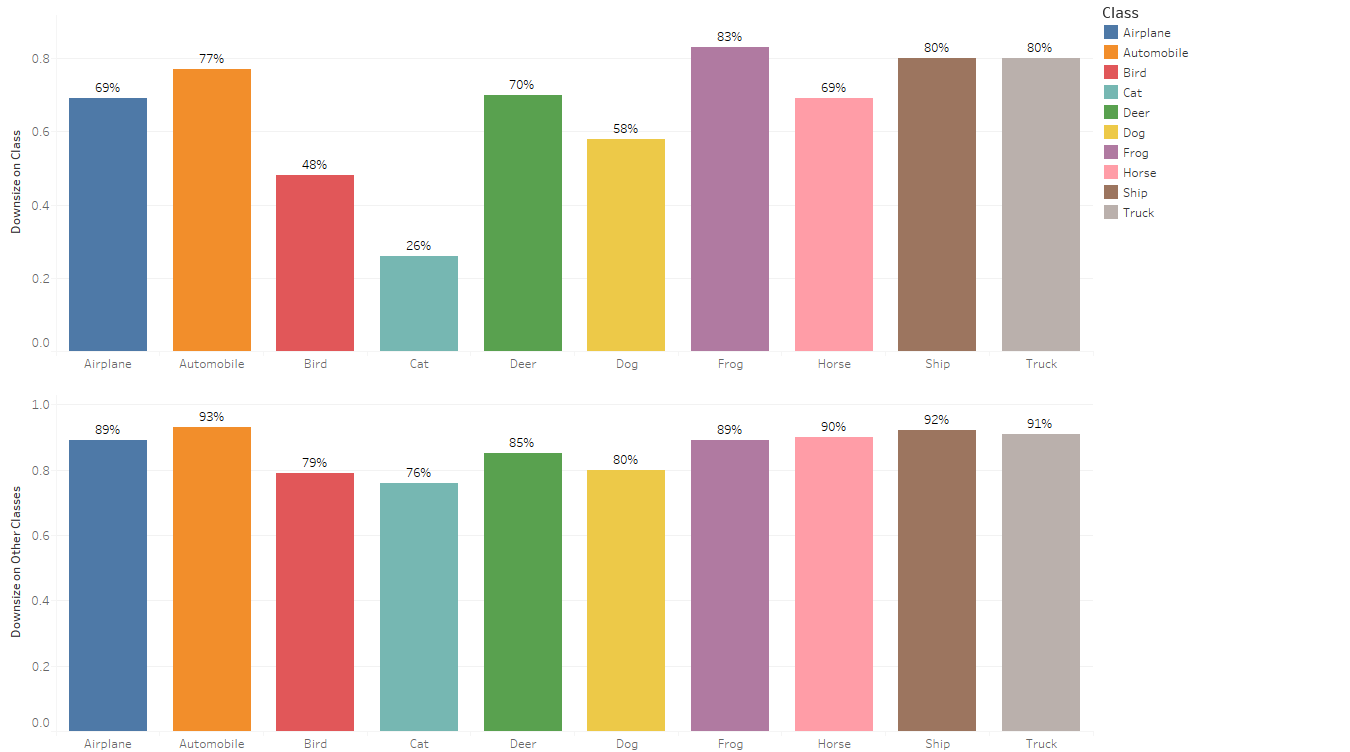
\includegraphics[scale=0.5]{downsize_graph.png}
	\caption{Target class accuracy on all the 20 per-class models}
	\label{fig:acc_graph}
\end{figure}

Figure ~\ref{fig:acc_graph} shows the per class accuracy for each specific model on non-perturbed test set. While the downsize on other classes causes the per class accuracy to increase, the downsize on class causes the same accuracy to be drastically reduced when compared to the balanced model shown on figure ~\ref{fig:conf_matrix}. The former happens because the model learns more about the target class due to its increased number samples, hence, it concentrates on learning the specifics of the class rather than equally splitting its capacity through all classes as it happens on the latter. The increased accuracy means that the model better explores the space around the target class since it does not have enough evidence to explore other classes spaces.

\section{Hypotheses formulations}
This work focuses on explaining the relationship between the data imbalance learning problem and adversarial attacks. Both subjects relate to each other as they are different ways of explaining the underlying data space exploration by the machine learning method. As datasets go into higher dimension, it becomes harder to the human rational to explain space transformations, as one usually is able to visualize only smaller dimensions of space. Specifically deep learning models are seen as "black box" due to its high complexity learning behavior. The hypotheses to explain the aforementioned relationship is as follows:

\begin{itemize}
	\item \textbf{(H1)} - Would adversarial attacks be more effective against models where the target of the attack is the minority class of the underlying training set ?
	\item \textbf{(H2)} - Would adversarial attacks be more effective against models where the target of the attack is the majority class of the underlying training set ?
	\item \textbf{(H3)} - Would adversarial attacks intensify the misclassification between classes with overlapping distributions ?
	\item \textbf{(H3)} - Would adversarial attacks on the minority classes make classification mistakes towards the majority class ?
\end{itemize}
